\documentclass[aspectratio=169]{beamer}

% ─── Theme ───
% Clean minimal theme — let the colors do the talking
\usetheme{default}
\useinnertheme{rounded}
\useoutertheme{default}

% ═══════════════════════════════════════════════════
% Kahawa Roots Brand Colors (matched to website)
% ═══════════════════════════════════════════════════
% Primary: #51624D green from website, coffee brown for accents, white everything else

% Primary brand colors
\definecolor{kahawaGreen}{RGB}{46, 91, 74}         % #2E5B4A — the main brand green (matched to website)
\definecolor{kahawaGreenDark}{RGB}{34, 70, 56}     % darker shade for hover/depth
\definecolor{kahawaBrown}{RGB}{101, 67, 33}       % coffee brown — subsections/accents
\definecolor{kahawaBrownLight}{RGB}{139, 100, 60} % lighter brown for subtle elements
\definecolor{kahawaWhite}{RGB}{255, 255, 255}     % clean white — backgrounds
\definecolor{textDark}{RGB}{51, 51, 51}           % #333 — clean professional dark text

% Utility colors (kept for diagrams)
\definecolor{gcpBlue}{RGB}{66, 133, 244}
\definecolor{bronzeColor}{RGB}{166, 80, 30}
\definecolor{silverColor}{RGB}{21, 101, 192}
\definecolor{goldColor}{RGB}{198, 134, 46}

% ═══════════════════════════════════════════════════
% Apply brand colors to Beamer elements
% ═══════════════════════════════════════════════════

% Background: clean white
\setbeamercolor{background canvas}{bg=kahawaWhite}

% Frame titles: brand green bar with white text
\setbeamercolor{frametitle}{bg=kahawaGreen, fg=kahawaWhite}
\setbeamertemplate{frametitle}{
    \vspace{0.15cm}
    \begin{beamercolorbox}[wd=\paperwidth, ht=0.7cm, dp=0.2cm, leftskip=0.5cm]{frametitle}
        \usebeamerfont{frametitle}\insertframetitle
    \end{beamercolorbox}
}

% Title page
\setbeamercolor{title}{fg=kahawaGreen}
\setbeamercolor{subtitle}{fg=kahawaBrown}
\setbeamercolor{author}{fg=textDark}
\setbeamercolor{institute}{fg=kahawaBrown}

% Blocks: green header, white body
\setbeamercolor{block title}{bg=kahawaGreen, fg=kahawaWhite}
\setbeamercolor{block body}{bg=kahawaWhite, fg=textDark}

% Alert blocks: brown header, white body
\setbeamercolor{block title alerted}{bg=kahawaBrown, fg=kahawaWhite}
\setbeamercolor{block body alerted}{bg=kahawaWhite, fg=textDark}

% Items: green bullets, brown sub-bullets
\setbeamercolor{item}{fg=kahawaGreen}
\setbeamercolor{subitem}{fg=kahawaBrown}
\setbeamercolor{itemize item}{fg=kahawaGreen}
\setbeamercolor{itemize subitem}{fg=kahawaBrown}
\setbeamercolor{description item}{fg=kahawaBrown}

% Normal text
\setbeamercolor{normal text}{fg=textDark, bg=kahawaWhite}

% Footer bar: green with white text
\setbeamercolor{footline}{bg=kahawaGreen, fg=kahawaWhite}

% ─── Fonts ───
\setbeamerfont{frametitle}{size=\large, series=\bfseries}
\setbeamerfont{title}{size=\LARGE, series=\bfseries}

% ─── Packages ───
\usepackage{graphicx}
\usepackage{booktabs}
\usepackage{fontawesome5}
\usepackage{hyperref}
\usepackage{listings}
\usepackage{xcolor}
\usepackage{tikz}
\usepackage{multicol}

% SQL code styling
\lstdefinestyle{sql}{
    language=SQL,
    basicstyle=\ttfamily\tiny,
    keywordstyle=\color{kahawaGreen}\bfseries,
    stringstyle=\color{kahawaBrown},
    commentstyle=\color{gray}\itshape,
    backgroundcolor=\color{kahawaWhite},
    frame=single,
    framerule=0.5pt,
    rulecolor=\color{kahawaBrownLight},
    breaklines=true,
    showstringspaces=false,
    tabsize=2
}

\hypersetup{
    colorlinks=true,
    linkcolor=kahawaBrown,
    urlcolor=gcpBlue
}

% ─── Title Info ───
\title[Kahawa Roots]{\textbf{Kahawa Roots} \\ \large Traceability Platform — Pre-Interview Task}
\subtitle{Tracking Coffee from Kenya's Farms to the UK}
\author{Shree Hari Anbazhagan}
\institute{Developer Intern Candidate}
\date{April 2026}

% ─── Remove navigation symbols ───
\setbeamertemplate{navigation symbols}{}

% ─── Slide numbers: brown bar footer ───
\setbeamertemplate{footline}{
    \begin{beamercolorbox}[wd=\paperwidth, ht=0.35cm, dp=0.15cm]{footline}
        \hfill{\scriptsize\color{kahawaWhite}\insertframenumber/\inserttotalframenumber}\hspace*{0.4cm}
    \end{beamercolorbox}
}

\begin{document}

% ══════════════════════════════════════════════════════════════
% SLIDE 1: TITLE + WHO I AM + PROOF
% ══════════════════════════════════════════════════════════════
\begin{frame}

\begin{columns}[T]

\begin{column}{0.55\textwidth}
    \vspace{1em}
    {\LARGE\textbf{\textcolor{kahawaBrown}{Kahawa Roots}}}\\[0.3em]
    {\large Traceability Platform}\\[0.1em]
    {\small\textit{Tracking Coffee from Kenya's Farms to the UK}}\\[1.5em]

    {\normalsize\textbf{Shree Hari Anbazhagan}}\\[0.5em]
    \begin{tabular}{@{}ll}
        \faEnvelope & \href{mailto:shreeharianbazhagan@gmail.com}{shreeharianbazhagan@gmail.com} \\
        \faPhone & 07721046613 \\
    \end{tabular}

    \vspace{1.5em}
    {\footnotesize\textcolor{gray}{Pre-Interview Task — Developer Intern — April 2026}}
\end{column}

\begin{column}{0.42\textwidth}
    \vspace{1em}
    \begin{block}{\faRocket\ Proof: I've Built This Before}
        \small
        My live full-stack project on the \textbf{same GCP infrastructure} I'm proposing:

        \vspace{0.3em}
        \begin{itemize}
            \item[\faGlobe] \scriptsize{\href{https://deltaed-frontend-93684845515.europe-west2.run.app}{\textcolor{gcpBlue}{DeltaEd — Live on GCP Cloud Run}}}
            \item[\faCloud] GCP Cloud Run, \texttt{europe-west2} (London)
            \item[\faDocker] Dockerized, full stack
            \item[\faCode] React + Next.js + PostgreSQL
        \end{itemize}

        \vspace{0.3em}
        \scriptsize{\textit{happy to walk through the architecture if interested.}}
    \end{block}
\end{column}

\end{columns}

\end{frame}

% ══════════════════════════════════════════════════════════════
% SLIDE 2: HOW I'D BUILD THIS + NON-TECHNICAL ACCESS
% ══════════════════════════════════════════════════════════════
\begin{frame}{Part 1 \& 3: How I'd Build This}

\begin{columns}[T]

\begin{column}{0.55\textwidth}

\textbf{\faDatabase\ How Data is Stored \& Recorded}
\begin{itemize}
    \item every shipment gets a unique ID when its first recorded
    \item raw data (form/CSV) goes straight into \textbf{GCP Cloud Storage} as a backup — never touched, never deleted
    \item a \textbf{Cloud Function} auto-triggers, cleans and validates the data
    \item clean data lands in \textbf{Cloud SQL (PostgreSQL)} — 3 tables: \texttt{farmers}, \texttt{shipments}, \texttt{shipment\_stages}
    \item each stage (farm → processing → export → UK) is a row in \texttt{shipment\_stages} with timestamps and GPS
\end{itemize}

\textbf{\faQrcode\ QR Code → Webpage}
\begin{itemize}
    \item QR is generated per shipment, encodes a URL like \texttt{/trace/SH-2026-001}
    \item scanning opens a public page with a \textbf{map} (Kenya → UK) + journey timeline + farmer details
\end{itemize}

\end{column}

\begin{column}{0.42\textwidth}

\textbf{\faUserFriends\ Non-Technical Data Entry (Part 3)}

\vspace{0.3em}
the founders (Rupal \& Cetric) aren't developers — so the system has two simple ways to add data:

\vspace{0.5em}
\begin{block}{\faWpforms\ Option 1: Web Form}
    \begin{itemize}
        \item fill in a simple form on the admin dashboard
        \item one shipment at a time
        \item no coding, no terminal, no SQL
    \end{itemize}
\end{block}

\begin{block}{\faFileExcel\ Option 2: CSV/Excel Upload}
    \begin{itemize}
        \item drag and drop a spreadsheet
        \item bulk import — great when cooperatives send batch data
        \item system validates every row automatically
    \end{itemize}
\end{block}

\vspace{0.3em}
\footnotesize{\textit{both options feed into the same REST API → same validation → same database. zero coding needed from the user.}}

\end{column}

\end{columns}

\end{frame}

% ══════════════════════════════════════════════════════════════
% SLIDE 3: TECHNOLOGY CHOICES + BONUS
% ══════════════════════════════════════════════════════════════
\begin{frame}{Part 2: Technology Choices + Bonus}

\begin{columns}[T]

\begin{column}{0.48\textwidth}

\textbf{\faTools\ Tech Stack \& Why}

\vspace{0.3em}
\footnotesize
\begin{tabular}{p{2.2cm} p{4.5cm}}
    \toprule
    \textbf{Component} & \textbf{Choice \& Why} \\
    \midrule
    \textbf{Cloud} & \textbf{GCP} (London region) \\
    & — \textcolor{kahawaGreen}{\textbf{up to \$200K startup credits}} \\
    & — UK data centre = GDPR friendly \\
    & — Cloud Run scales to zero = pay nothing when idle \\
    \midrule
    \textbf{Backend} & \textbf{Python + REST API} on Cloud Run \\
    & — fast to build, great for data validation \\
    \midrule
    \textbf{Frontend} & \textbf{Next.js (React)} on Cloud Run \\
    & — SSR for fast QR page loads, SEO friendly \\
    \midrule
    \textbf{Database} & \textbf{Cloud SQL (PostgreSQL)} \\
    & — relational, sub-10ms reads for QR scans \\
    \midrule
    \textbf{Storage} & \textbf{Cloud Storage} buckets \\
    & — immutable raw data backup \\
    \midrule
    \textbf{Processing} & \textbf{Cloud Functions} \\
    & — event-driven, auto-triggered on new data \\
    \midrule
    \textbf{IaC} & \textbf{Terraform} — infra as code, repeatable \\
    \midrule
    \textbf{CI/CD} & \textbf{GitHub Actions} — auto deploy on push \\
    \midrule
    \textbf{Maps} & \textbf{Google Maps API} — native to GCP \\
    \bottomrule
\end{tabular}

\end{column}

\begin{column}{0.48\textwidth}

\textbf{\faLayerGroup\ Data Architecture: Medallion Pattern}

\vspace{0.3em}
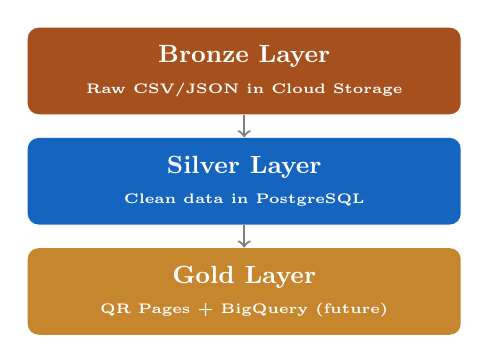
\begin{tikzpicture}[
    layer/.style={rounded corners=4pt, minimum width=5.5cm, minimum height=1.1cm, text=white, font=\small\bfseries, align=center},
    arrow/.style={->, thick, gray}
]
    \node[layer, fill=bronzeColor] (bronze) at (0,3) {Bronze Layer \\ \tiny Raw CSV/JSON in Cloud Storage};
    \node[layer, fill=silverColor] (silver) at (0,1.6) {Silver Layer \\ \tiny Clean data in PostgreSQL};
    \node[layer, fill=goldColor] (gold) at (0,0.2) {Gold Layer \\ \tiny QR Pages + BigQuery (future)};

    \draw[arrow] (bronze) -- (silver);
    \draw[arrow] (silver) -- (gold);
\end{tikzpicture}

\vspace{0.5em}
\vspace{0.5em}
\textbf{\faCode\ Bonus: Database Schema}

{\ttfamily\tiny\color{textDark}
\begin{tabular}{@{}l@{}}
\textcolor{kahawaGreen}{\textbf{CREATE TABLE}} farmers ( \\
\quad id \quad\quad UUID PRIMARY KEY, \\
\quad name \quad VARCHAR(100), \\
\quad region \quad VARCHAR(100), \\
\quad farm\_size DECIMAL, \\
\quad latitude \quad DECIMAL(9,6), \\
\quad longitude DECIMAL(9,6), \\
\quad cooperative VARCHAR(100) \\
); \\[0.3em]
\textcolor{kahawaGreen}{\textbf{CREATE TABLE}} shipments ( \\
\quad id \quad\quad UUID PRIMARY KEY, \\
\quad batch\_id VARCHAR(50) UNIQUE, \\
\quad farmer\_id UUID REFERENCES farmers(id), \\
\quad grade \quad VARCHAR(10), \\
\quad weight\_kg DECIMAL, \\
\quad status \quad VARCHAR(20), \\
\quad created\_at TIMESTAMP DEFAULT NOW() \\
); \\[0.3em]
\textcolor{kahawaGreen}{\textbf{CREATE TABLE}} shipment\_stages ( \\
\quad id \quad\quad\quad UUID PRIMARY KEY, \\
\quad shipment\_id UUID REFERENCES shipments(id), \\
\quad stage \quad\quad VARCHAR(50), \\
\quad location \quad VARCHAR(100), \\
\quad notes \quad\quad TEXT \\
); \\
\end{tabular}
}

\end{column}

\end{columns}

\end{frame}

% ══════════════════════════════════════════════════════════════
% SLIDE 4: FULL ARCHITECTURE DIAGRAM
% ══════════════════════════════════════════════════════════════
\begin{frame}{System Architecture}

\begin{center}

% ── Replace this with your screenshot ──
% 1. Export your draw.io diagram as PNG (File → Export as → PNG, 2x scale)
% 2. Save as "architecture.png" in the same folder as this .tex file
% 3. Uncomment the line below and delete the placeholder box

% 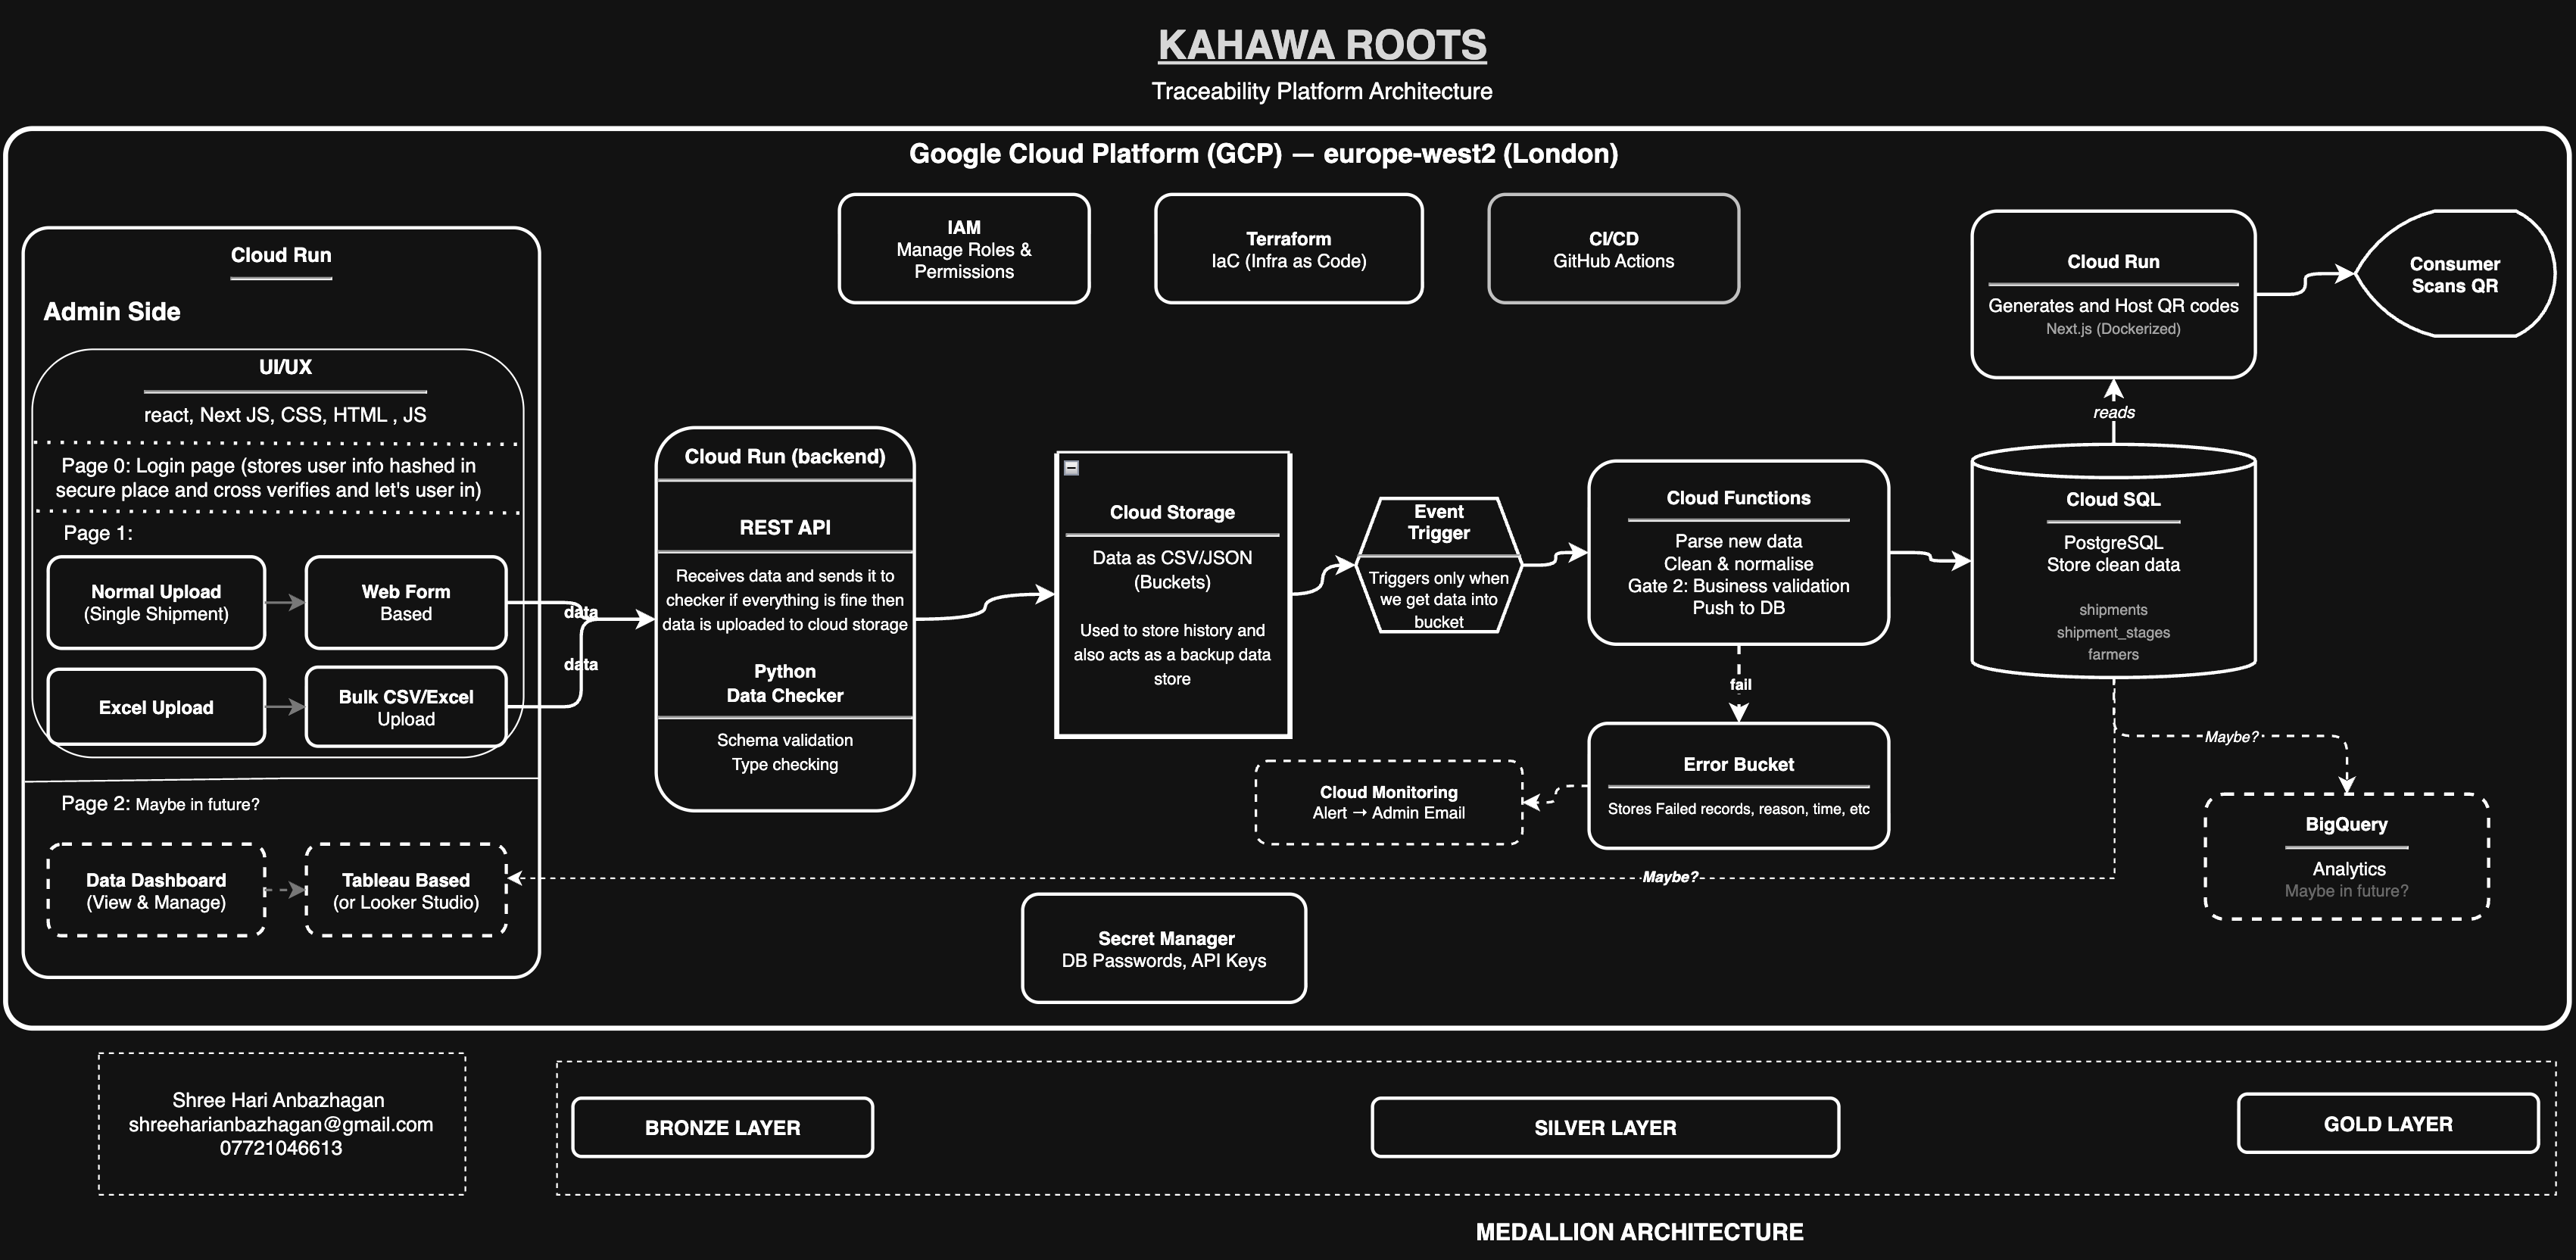
\includegraphics[width=\textwidth,height=0.78\textheight,keepaspectratio]{architecture.png}

% ── PLACEHOLDER — delete this block after adding your image ──
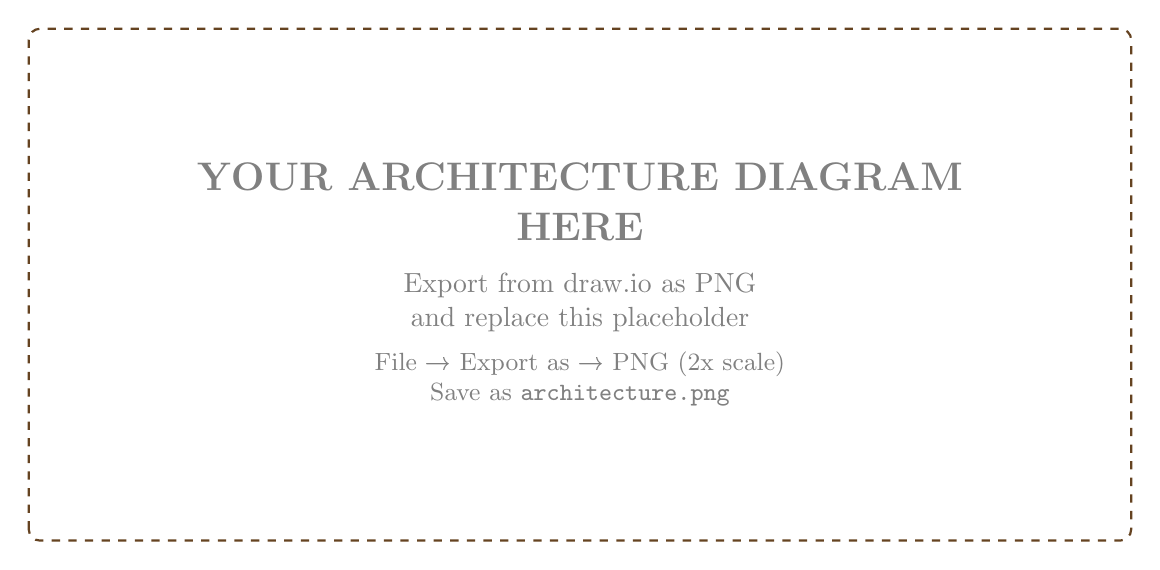
\begin{tikzpicture}
    \draw[kahawaBrown, thick, dashed, rounded corners] (0,0) rectangle (14,6.5);
    \node[text=gray, font=\Large] at (7,3.25) {
        \parbox{10cm}{\centering
            \textbf{YOUR ARCHITECTURE DIAGRAM HERE}\\[0.5em]
            \normalsize Export from draw.io as PNG\\
            and replace this placeholder\\[0.5em]
            \small File → Export as → PNG (2x scale)\\
            Save as \texttt{architecture.png}
        }
    };
\end{tikzpicture}
% ── END PLACEHOLDER ──

\end{center}

\vspace{-0.3em}
{\footnotesize \textcolor{gcpBlue}{\faLink\ \href{https://viewer.diagrams.net/?tags=\%7B\%7D&lightbox=1&highlight=0000ff&edit=_blank&layers=1&nav=1&title=kahawa-roots-architecture.drawio&dark=auto}{Click here for interactive architecture diagram}}}

\end{frame}

% ══════════════════════════════════════════════════════════════
% SLIDE 5: WHAT DOES ALL THIS MEAN? (Plain English)
% ══════════════════════════════════════════════════════════════
\begin{frame}{What Does All This Actually Mean?}

\begin{columns}[T]

\begin{column}{0.48\textwidth}

\textbf{\faCubes\ Architecture Concepts}
\vspace{0.3em}

\begin{description}[leftmargin=0pt, labelwidth=0pt, font=\small\bfseries\color{kahawaBrown}]

    \item[Microservices] \scriptsize instead of one big application, we split into 3 small independent apps — admin panel, backend API, and QR page. if one breaks or needs updating, the others keep running. like separate kitchens in a restaurant.

    \item[Cloud Functions] \scriptsize a small piece of code that runs \textit{only} when new data arrives in storage. no server to manage, no cost when idle. think of it like a light that turns on only when someone walks in.

    \item[REST API] \scriptsize the ``messenger'' between the admin form and the database. when you submit data, the API checks it, cleans it, and passes it along. like a receptionist who filters visitors before they enter.

    \item[PostgreSQL] \scriptsize a database — like a very smart spreadsheet. it stores all shipment data in organised tables with relationships. e.g. each shipment links to a farmer, each farmer has stages.

    \item[Medallion Architecture] \scriptsize data goes through 3 layers: \textcolor{bronzeColor}{\textbf{Bronze}} (raw, untouched backup) → \textcolor{silverColor}{\textbf{Silver}} (cleaned and validated) → \textcolor{goldColor}{\textbf{Gold}} (ready for customers to see). ensures no bad data ever reaches the QR page.

\end{description}

\end{column}

\begin{column}{0.48\textwidth}

\textbf{\faLock\ Operations \& Security}
\vspace{0.3em}

\begin{description}[leftmargin=0pt, labelwidth=0pt, font=\small\bfseries\color{kahawaBrown}]

    \item[IAM (Identity \& Access)] \scriptsize controls \textit{who} can do \textit{what}. e.g. admins can add shipments, but the public can only view QR pages. like a key card system in an office — different doors for different people.

    \item[Terraform (IaC)] \scriptsize instead of clicking buttons to set up servers manually, we write a config file that does it automatically. if we need to rebuild everything, one command recreates the whole system. like a recipe vs cooking from memory.

    \item[CI/CD (GitHub Actions)] \scriptsize every time we push code, it's automatically tested and deployed. no manual uploads, no ``it works on my laptop'' problems. like an assembly line for software.

    \item[Secret Manager] \scriptsize stores passwords and API keys securely. nobody can accidentally see or leak database credentials. like a safe inside the server room.

\end{description}

\vspace{0.5em}

\textbf{\faChartLine\ Future Plans}
\vspace{0.3em}

\begin{description}[leftmargin=0pt, labelwidth=0pt, font=\small\bfseries\color{kahawaBrown}]

    \item[BigQuery] \scriptsize when we have enough data — analytics. ``which region produces the fastest shipments?'' or ``average transit time trends''. not needed now, but the architecture is ready for it.

    \item[Data Dashboard] \scriptsize a visual dashboard (Tableau/Looker Studio) for founders to see charts and trends without touching the database. planned once there's enough shipment history.

\end{description}

\end{column}

\end{columns}

\end{frame}

\end{document}
